\chapter{Connections}\label{ch:connections}
Many musical instruments consist of multiple subsystems like the ones presented in Part \ref{part:resonators}. For example, one could simulate a guitar by modelling six separate instances of the stiff string presented in Chapter \ref{ch:stiffString}, and the sound board (as a simplified instrument body), using a thin plate presented in Section \ref{sec:thinPlate}. 
The interaction between the strings and the body can then be modelled using \textit{connections}. %Apart from interactions between resonators, one could use connections for instrument control. For example, one could connect a mass-spring-damper system to a string, to simulate a point-like damping finger to create different pitches.

Examples of connected resonators based on FDTD methods are shown in e.g. \cite{theBible} and \cite{Bilbao2009Modular}. The latter presents a modular approach to connect any number of resonators in arbitrary ways using an extremely compact matrix form of the entire system.
% Although briefly mentioned in the previous chapter in Section \ref{sec:twoSidedCollision}

The first example presented in this chapter is the case of two ideal strings, connected using a rigid and spring-like connection. Afterwards, the connection between a stiff string and a thin plate using a nonlinear spring will be presented, and has been used extensively in papers \citeP[A] and \citeP[B]. Before moving on to these examples, interpolation and spreading operators in 2D will be introduced.

\section{Interpolation and spreading in 2D}\label{sec:interpolationSpreading2D}
This section summarises and extends \cite[Sec. 10.2.1, pp. 293--294]{theBible}.

One can extend the interpolation and spreading operators presented in Section \ref{sec:interpolationSpreading} to 2D by adding an additional argument to the operators. Using $l_\itxt = \floor[x_\itxt / h]$ and $m_\itxt = \floor[y_\itxt / h]$, a $0$\thOrder interpolation operator $I_0(x_\itxt, y_\itxt) = I_{(l, m), 0}(x_\itxt, y_\itxt)$ is defined as
\begin{equation}
    I_0(x_\itxt, y_\itxt) = \begin{cases}
        1, & \text{if } l = l_\itxt \text{ and } m = m_\itxt,\\
        0, & \text{otherwise}.
    \end{cases}
\end{equation}
Notice that the same value for the grid spacing $h$ is used for both the $x$ and $y$ direction.

Using the fractional part of the flooring operations $\alpha_x = x_\itxt/h - l_\itxt$ and $\alpha_y= y_\itxt/h - m_\itxt$, a 2D linear interpolator  $I_1(x_\itxt, y_\itxt) = I_{(l, m), 1}(x_\itxt, y_\itxt)$ can then be composed as
\begin{equation}
    I_1(x_\itxt, y_\itxt) = \begin{cases}
        (1 - \alpha_x)(1 - \alpha_y)& \text{if } l = l_\itxt \text{ and } m = m_\itxt, \\
        (1 - \alpha_x)\alpha_y& \text{if } l = l_\itxt \text{ and } m = m_\itxt + 1, \\
        \alpha_x(1 - \alpha_y)& \text{if } l = l_\itxt + 1 \text{ and } m = m_\itxt, \\
        \alpha_x\alpha_y& \text{if } l = l_\itxt+1 \text{ and } m = m_\itxt+1, \\
        0, & \text{otherwise}.
    \end{cases}
\end{equation}

Spreading operators are defined in the same way as in Section \ref{sec:interpolationSpreading}. A $0$\thOrder spreading operator $J_0(x_\itxt, y_\itxt) = J_{(l,m),0}(x_\itxt, y_\itxt)$ can be defined as
\begin{equation}
    J_0(x_\itxt, y_\itxt) = \frac{1}{h^2}\begin{cases}
        1, & \text{if } l = l_\itxt \text{ and } m = m_\itxt,\\
        0, & \text{otherwise},
    \end{cases}
\end{equation}
as well as a linear spreading operator $J_1(x_\itxt, y_\itxt) = J_{(l,m),1}(x_\itxt, y_\itxt)$ as
\begin{equation}
    J_1(x_\itxt, y_\itxt) = \frac{1}{h^2}\begin{cases}
        (1 - \alpha_x)(1 - \alpha_y)& \text{if } l = l_\itxt \text{ and } m = m_\itxt, \\
        (1 - \alpha_x)\alpha_y& \text{if } l = l_\itxt \text{ and } m = m_\itxt + 1, \\
        \alpha_x(1 - \alpha_y)& \text{if } l = l_\itxt + 1 \text{ and } m = m_\itxt, \\
        \alpha_x\alpha_y& \text{if } l = l_\itxt+1 \text{ and } m = m_\itxt+1, \\
        0, & \text{otherwise}.
    \end{cases}
\end{equation}
Notice that the scaling is by $1/h^2$ (due to the 2D system) rather than $1/h$ in the 1D case. Some intuition on this will be given below. 

As in the 1D case, the spreading operator approximates a spatial Dirac delta function, which -- in 2D -- is defined as 
\begin{equation}\label{eq:spatialDirac2D}
    \delta(x,y)= \begin{cases}
        \infty, & x = y = 0,\\
        0, & \text{otherwise},
    \end{cases} \qaq \int_{-\infty}^{\infty} \int_{-\infty}^{\infty} \delta(x,y)dxdy = 1.
\end{equation}
where $\delta(x,y)$ has units of m$^{-2}$. Again, as described in Section \ref{sec:interpolationSpreading}, this definition will be approximated by spreading operators, rather than be used directly. 

\subsection{Alternative interpretation of grid points}\label{sec:alternativeInterp}
Section \ref{sec:gridFunctions} gives an introduction to how a continuous 1D system is subdivided into grid points in space (see Figure \ref{fig:gridExp}) through the discretisation process. An alternative way to see grid points after discretisation is shown in Figure \ref{fig:gridExp2}. Rather than grid `points' with a spacing $h$ between them, a continuous system is divided into grid `sections' of length $h$. This interpretation allows for the `weight' of a grid point to be calculated from its material properties and geometry. Notice that boundaries have a length of $h/2$ such that the total length $L = Nh$ m.

As an example, the weight of one grid point (or now rather grid section) of a string can be calculated as $\rho A h$. The weight of one grid point of a 2D system can be calculated as $\rho H h^2$. As these grid points interact with each other, the forces resulting from this interaction will be scaled by their respective weight per grid point as will be shown in Section \ref{sec:stringPlateConnection}.
This interpretation hopefully provides a better intuition for the interactions between components shown in this chapter. 

\begin{figure}[h]
    \centering
    % \subfloat[If $N=5$ there are 5 sections of length $h$ and 6 grid points describing the state of the system ($l=\{0, \hdots, 5\}$).\label{fig:gridExp1}]{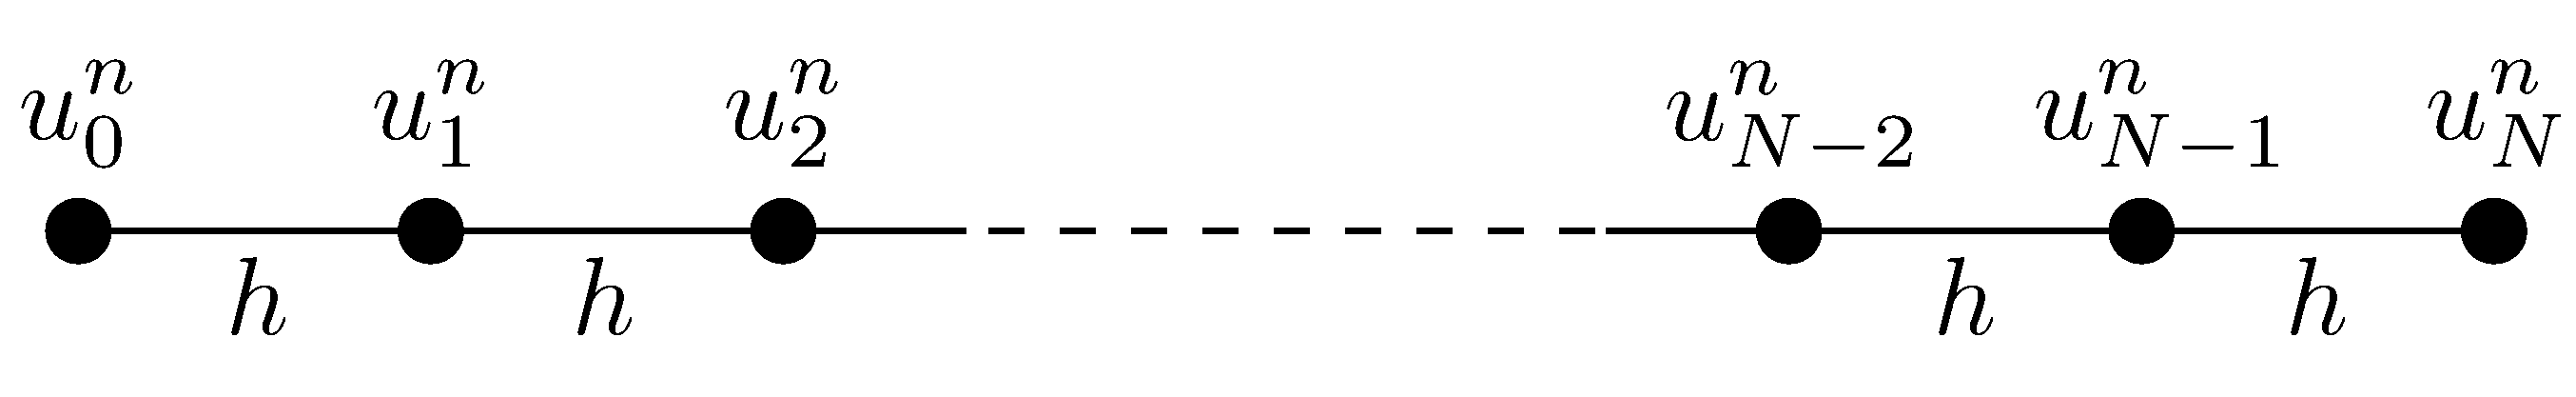
\includegraphics[width=0.45\textwidth]{figures/fdtd/gridExplanation.pdf}}\hspace{0.06\textwidth}
    % \subfloat[If $N$ is large (as is usually the case), The 1D system is divided into $N$ sections of length $h$ and $l=\{0, \hdots, N\}$.\label{fig:gridExp2}]{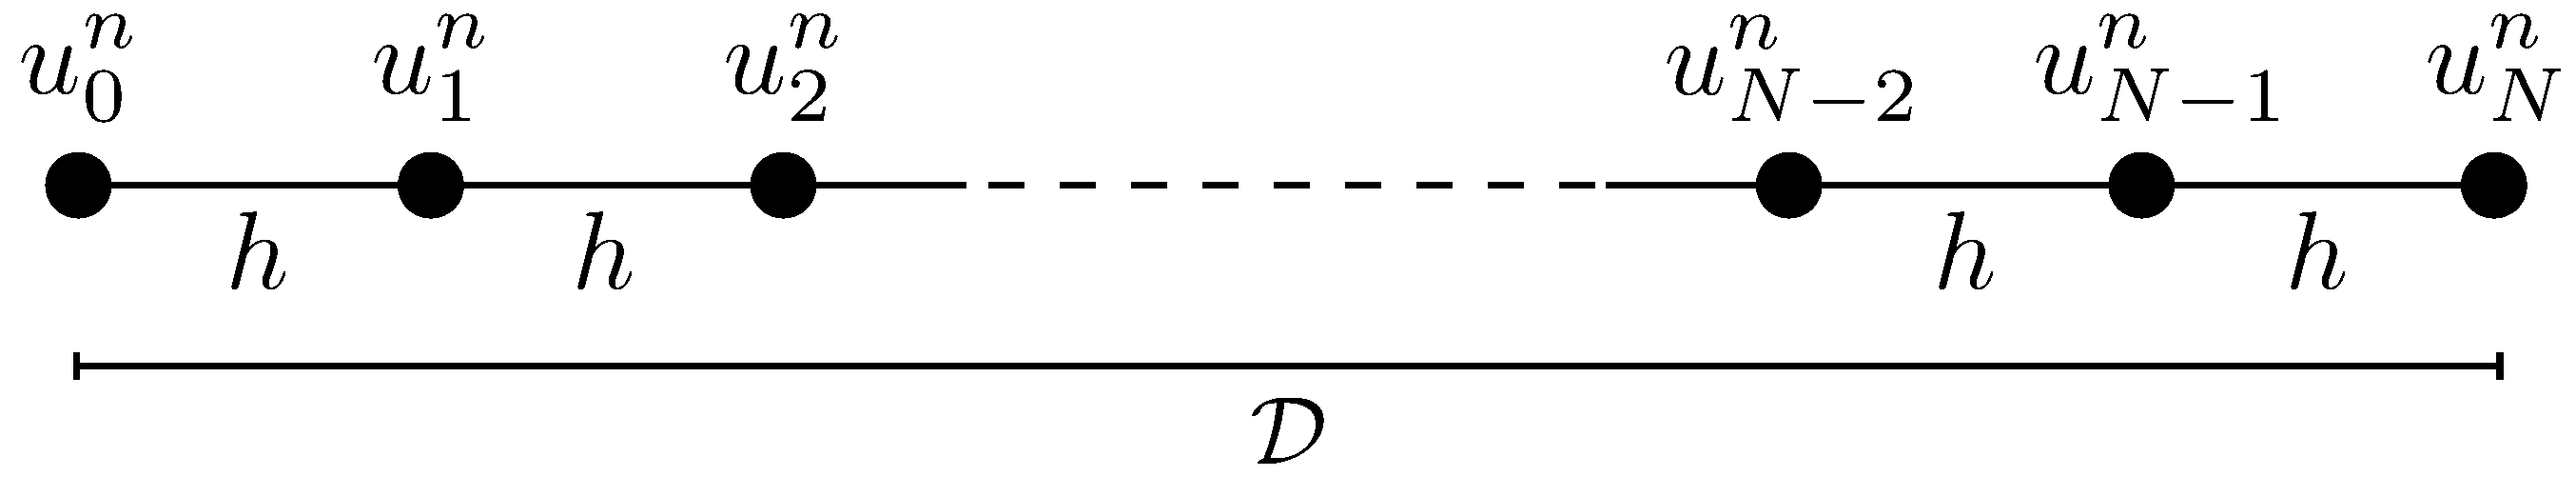
\includegraphics[width=0.45\textwidth]{figures/fdtd/gridExplanation2.pdf}}
    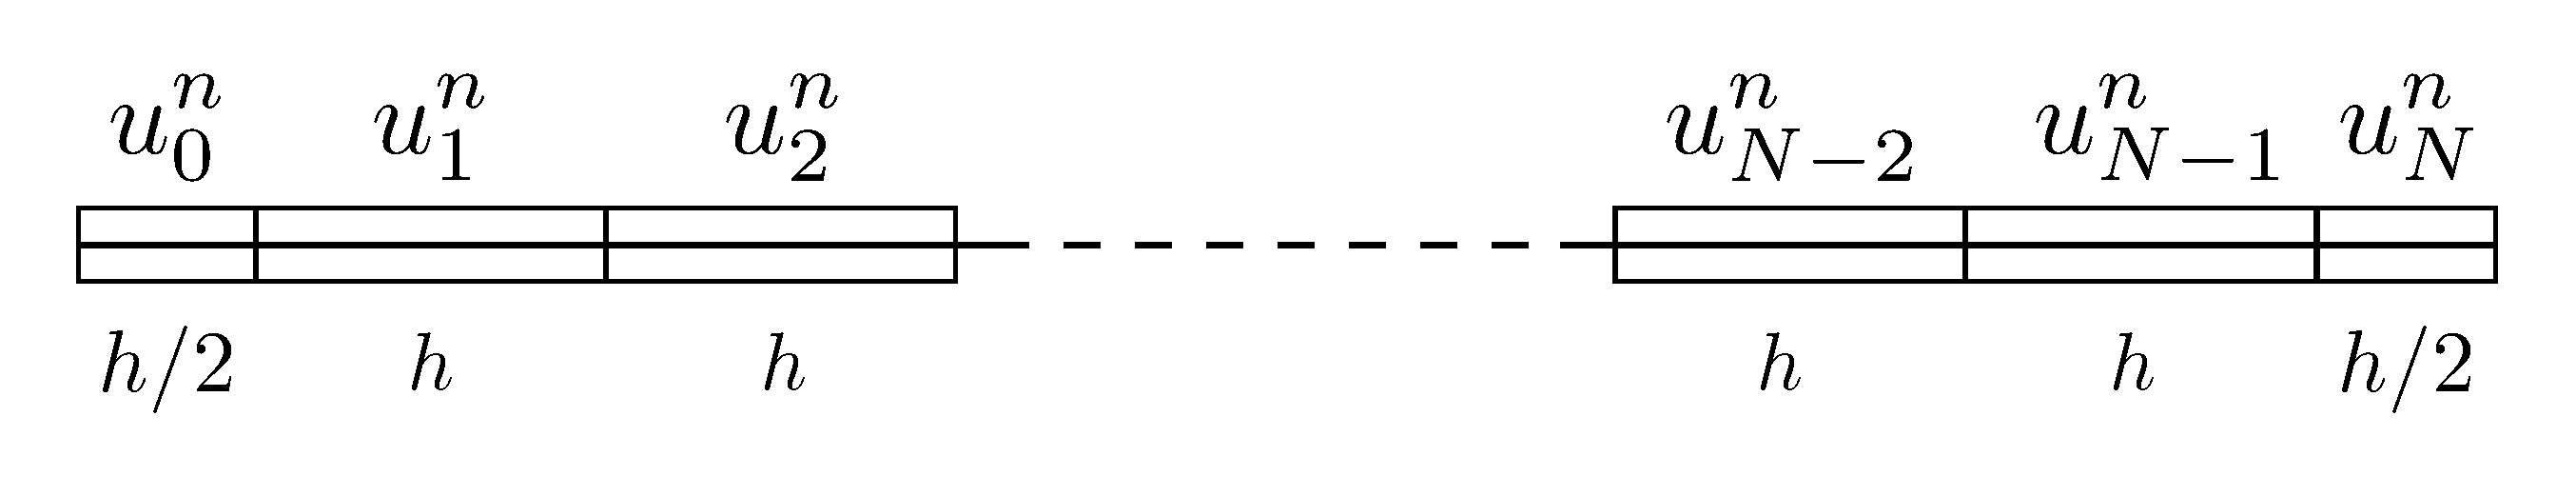
\includegraphics[width=0.75\textwidth]{figures/fdtd/gridFigure2.pdf}
    \caption{Alternative interpretation of the discretisation of $u(x,t)$ to a grid function $\uln$. The continuous system is divided into $N-1$ sections of length $h$ plus $2$ sections of length $h/2$ at the boundaries. Through this interpretation, the `weight' of a grid point can be calculated from its physical parameters. \label{fig:gridExp2}}
\end{figure}

\section{Connected ideal strings}\label{sec:connIdealStrings}
When working with multiple interacting systems, one finds that notation becomes extremely important. Subscripts will be extensively used in the following for extra clarity, and although this results in something of a notational jungle, it is better to be explicit and avoid confusion in the end.

As a test case for the following sections, consider two ideal strings\footnote{Recall that the ideal string is the 1D wave equation with $c=\sqrt{T/\rho A}$.} of length $L_u$ and $L_w$ (both in m) their transverse displacement denoted as $u=u(x,t)$ and $w = w(\chi,t)$ (both in m) respectively (see Section \ref{sec:1DWave}).  The systems are defined for $x\in \D_u$ with domain $\D_u=[0,L_u]$ and $\chi \in \D_w$ with domain $\D_w=[0,L_w]$ respectively. Notice that $\chi$ is used as the spatial coordinate for $w$ to denote that the two systems use different coordinate systems. Connecting these systems at $x_\ctxt\in \D_u$ and $\chi_\ctxt\in\D_w$ yields the following system of PDEs:
\begin{subequations}\label{eq:conn1DwavePDE}
    \begin{align}
        \rho_u A_u \ptt u &= T_u \pxx u -\delta(x-x_\ctxt)f, \label{eq:conn1DwavePDEu} \\
        \rho_w A_w \ptt w &= T_w \partial_\chi^2 w + \delta(\chi-\chi_\ctxt)f,\label{eq:conn1DwavePDEw}
    \end{align}
\end{subequations}
where subscripts $u$ and $w$ denote whether a variable belongs to system $u$ or $w$ respectively. Notice that the $\partial_\chi$ in Eq. \eqref{eq:conn1DwavePDEw} denotes a partial derivative with respect to $\chi$ and is an identical operation to $\px$, but on a different coordinate system. Furthermore, $f = f(t)$ is the connection force (in N) which should be equal and opposite for the connected systems according to Newton's third law (hence the inverse signs). The definition for $f$ depends on the connection type, and two alternatives will be given shortly. Finally, the spatial Dirac delta function $\delta$ is defined as in Eq. \eqref{eq:spatialDirac}, and localises the connection force along the systems. 
% The relative displacement between the two systems at their respective connection locations (in m) is defined as 
% \begin{equation}
%     \eta(t) = u(x_\text{c},t) - w_(\chi_\ctxt),
% \end{equation}
% and will be used later on. 

\subsubsection{Relative location of objects}
As explained in Chapter \ref{ch:collisions} it is important to keep in mind the relative location of two interacting objects, as this will affect the signs of the force terms added to the PDEs. As opposed to the case of collisions, the connection will have a negative effect on the object `above' and a positive effect on the one `below' due to the `pulling' behaviour of a connection.
From the signs of the force terms in system \eqref{eq:conn1DwavePDE}, it can thus be concluded that $u$ has been placed above $w$. If $f$ is positively dependent on $\eta$ (the relative displacement between the two objects at their respective connection locations), this will be defined as the object below subtracted from the object above. For system \eqref{eq:conn1DwavePDE} this will be
\begin{equation}
    \eta(t) = u(x_\text{c}, t) - w(\chi_\text{c}, t),
\end{equation}
and will be used for a spring connection in Section \ref{sec:springConnection}.

\subsection{Discrete time}
One can then discretise the state variables $u$ and $w$ to grid functions $\uln$ and $\wmn$, using $x = lh_u$ and $\chi = mh_w$, where $l\in \{0, \hdots, N_u\}$ and $m\in \{0, \hdots, N_w\}$.\footnote{Here, $m$ is used for the spatial index of $\wmn$ to avoid double subscripts $l_u$ and $l_w$.} Also see Section \ref{sec:gridFunctions}. Furthermore, $h_u$ and $h_w$ are the values of the grid spacing (both in m) and $N_u+1$ and $N_w+1$ are the number of grid points for $\uln$ and $\wmn$ respectively. Dividing Eqs. \eqref{eq:conn1DwavePDEu} and \eqref{eq:conn1DwavePDEw} by $\rho_u A_u$ and $\rho_w A_w$ respectively, yields
\begin{subequations}\label{eq:conn1DwaveFDS}
    \begin{align}
        \dtt \uln &= c_u^2 \dxx \uln -\Ju\frac{f^n}{\rho_u A_u}, \label{eq:conn1DwaveFDSu} \\
        \dtt \wmn &= c_w^2 \delta_{\chi\chi} \wmn + \Jw\frac{f^n}{\rho_w A_w},\label{eq:conn1DwaveFDSw}
    \end{align}
\end{subequations}
where $c_u = \sqrt{T_u / \rho_uA_u}$ and $c_w = \sqrt{T_w / \rho_wA_w}$. The spreading operators $\Ju = J_{l, o_u, u}(x_\ctxt)$ and $J_{l, w}(\chi_\ctxt) = J_{l, o_w, w}(\chi_\ctxt)$ are as defined in Section \ref{sec:interpolationSpreading}, and their orders $o_u$ and $o_w$ are left unspecified.

The next step would be to solve for connection force $f^n$. First, one needs to isolate the schemes in system \eqref{eq:conn1DwaveFDS} at their respective connection locations $x_\ctxt$ and $\chi_\ctxt$. This is done by taking an inner product of each scheme in system \eqref{eq:conn1DwaveFDS} with their respective spreading operator $J_{l, u}(x_\ctxt)$ and $J_{l, w}(\chi_\ctxt)$ over discrete domains $d_u = \{0, \hdots, N_u\}$ and $d_w = \{0, \hdots, N_w\}$ respectively. Using identity \eqref{eq:identityIJ} one can write
\begin{subequations}\label{eq:conn1DwaveFDSXc}
    \begin{align}
        \Iu\dtt \uln &= c_u^2 \Iu\dxx \uln -\lVert \Ju\rVert_{d_u}^2\frac{f^n}{\rho_u A_u}, \label{eq:conn1DwaveuXc} \\
        \Iw\dtt \wmn &= c_w^2 \Iw\delta_{\chi\chi} \wmn + \lVert \Jw\rVert_{d_w}^2\frac{f^n}{\rho_w A_w}.\label{eq:conn1DwavewXc}
    \end{align}
\end{subequations}
Here, interpolation operators $\Iu = I_{l, o_u, u}(x_\ctxt)$ and $\Iw = I_{l, o_w, w}(\chi_\ctxt)$ are as defined in Section \ref{sec:interpolationSpreading}. Notice that the order of these operators need 
to match their `dual' spreading operator, but the orders $o_u$ and $o_w$ may differ.

The definition of the force depends on the connection type. Below, two alternatives will be presented: the rigid connection and the spring connection. 

\section{Rigid connection}\label{sec:rigidConn}
The simplest connection-type is the \textit{rigid connection}. This connection type states that the displacement of two connected points should always be equal, and thus the distance between them should be 0 at all times. 
For the rigid connection, the following is true:
\begin{equation}\label{eq:contRigid}
    u(x_\ctxt, t) = w(\chi_\ctxt, t),
\end{equation}
which in discrete time becomes
\begin{equation}\label{eq:discRigid}
    \Iu\uln = \Iw\wmn.
\end{equation}
For a rigid connection, the following must also hold:
\begin{equation}\label{eq:discAccelRigid}
    \Iu\dtt\uln = \Iw\dtt\wmn.
\end{equation}
In other words, if the displacement of two objects is equal, their acceleration must also be. This definition can then immediately be used to solve for $f^n$ and the right-hand sides in system \eqref{eq:conn1DwaveFDSXc} can be substituted in Eq. \eqref{eq:discAccelRigid} to get
\begin{equation*}
    c_u^2 \Iu\dxx \uln -\lVert \Ju\rVert_{d_u}^2\frac{f^n}{\rho_u A_u}
    \!=\! c_w^2 \Iw\delta_{\chi\chi} \wmn + \lVert \Jw\rVert_{d_w}^2\frac{f^n}{\rho_w A_w},
\end{equation*}
which can be explicitly solved for $f^n$ according to
\begin{equation}\label{eq:rigidForce}
    f^n = \frac{c_u^2 \Iu\dxx \uln - c_w^2 \Iw\delta_{\chi\chi} \wmn}{\frac{\lVert \Ju\rVert_{d_u}^2}{\rho_u A_u} + \frac{\lVert \Jw\rVert_{d_w}^2}{\rho_w A_w}}\ .
\end{equation}
This value can then be used in the update equation obtained after expanding system \eqref{eq:conn1DwaveFDS} as
\begin{subequations}
    \begin{align}
        \!\!\!u_l^{n+1} &= \left(2-2\lambda_u^2\right) \uln  + \lambda_u^2\left(u_{l+1}^n + u_{l-1}^n\right) - u_l^{n-1} -\Ju\frac{k^2 f^n}{\rho_u A_u},\\
        \!\!\!w_m^{n+1} &= \left(2-2\lambda_w^2\right) \wmn\! +\! \lambda_w^2\left(w_{m+1}^n\! +\! w_{m-1}^n\right) \! -\! w_m^{n-1} +\Jw\frac{k^2 f^n}{\rho_w A_w},
    \end{align}
\end{subequations}
where $\lambda_u = c_uk/h_u \leq 1$ and  $\lambda_u = c_uk/h_u \leq 1$ are the Courant numbers for each individual scheme (see Section \ref{sec:1DWave}).

Figure \ref{fig:connectedWaveEqs} shows an implementation of system \eqref{eq:conn1DwaveFDS} with $x_\ctxt = 0.25$ m and $\chi_\ctxt = 0.75$ m. The ideal strings have the same mass per unit length, i.e., $\rho_uA_u = \rho_wA_w$, and the same length $L_u=L_w = 1$ m, but operate at different wave speeds $c_u=300$ m/s and $c_w=400$ m/s. The offset between the systems is made for clarity, and the locations connected by the grey line should have the same displacement as posed by the rigid connection. 

\begin{figure}[h]
    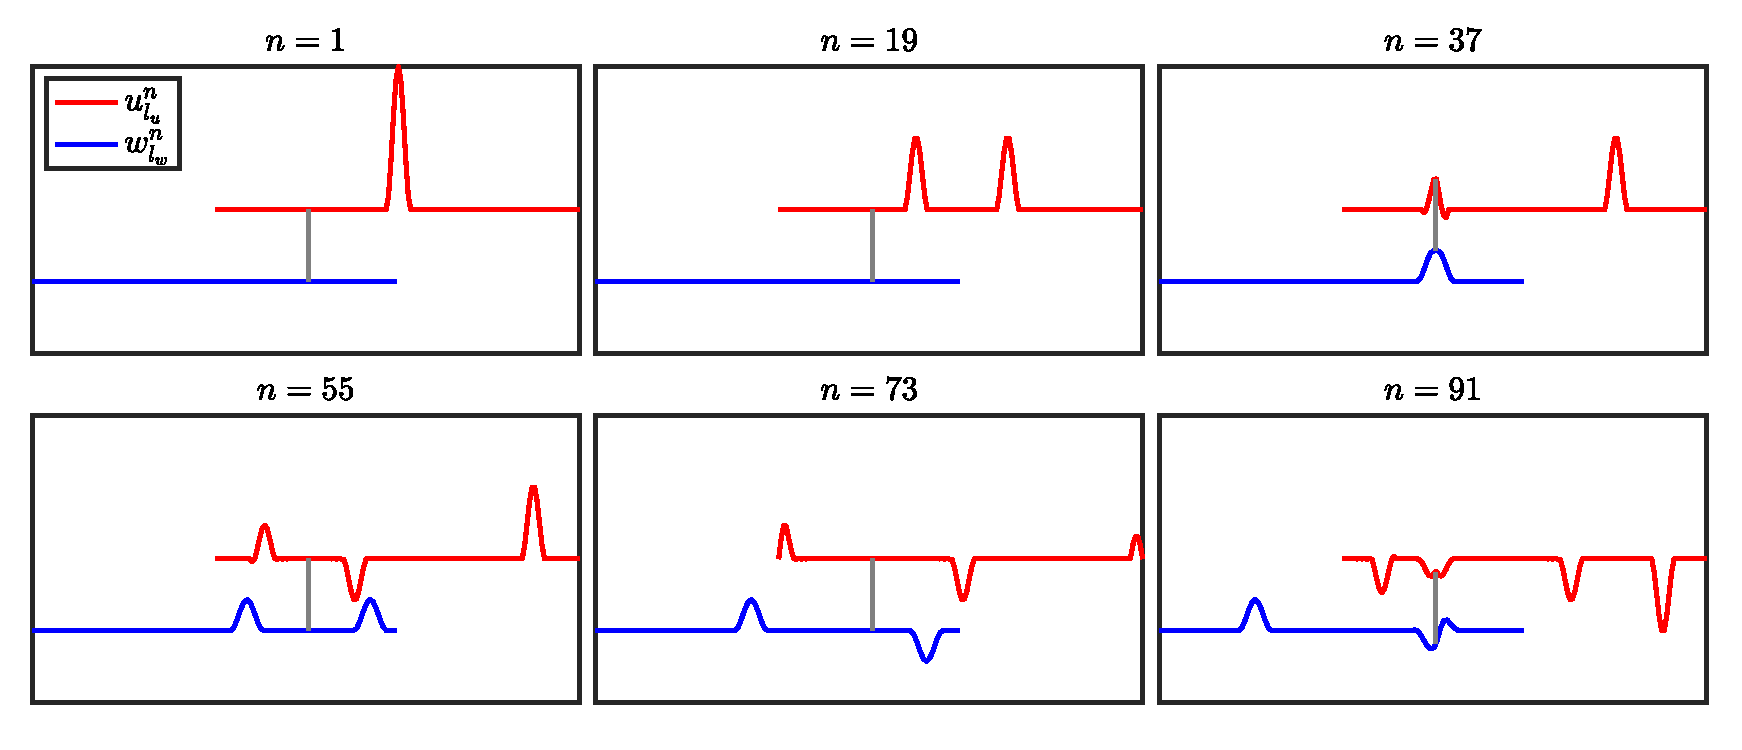
\includegraphics[width=\textwidth]{figures/interactions/connectedWaveEqs.eps}
    \caption{The behaviour of two connected 1D wave equations. The systems are offset for clarity, but the relative displacement at the connection location is 0. \label{fig:connectedWaveEqs}}
\end{figure}

\subsection{Notation simplification}\label{sec:notationSimplification}
In the above equations, the orders of the spreading and interpolation operators have been left unspecified to retain generality. If one would like to connect two systems at specified grid points (so not in-between), the notation can be greatly simplified.%\footnote{The same can be achieved if the orders of the interpolation and spreading operators are chosen to be 0, or if $\alpha_\itxt = 0$ for arbitrary orders.}

Recalling that $\Iu = I_{l, o_u, u}(x_\ctxt)$ and $\Iw = I_{l, o_w, w}(\chi_\ctxt)$, one can set the interpolation orders to 0, i.e., $o_u = o_w = 0$, to yield the following short-hand notations
\begin{equation}\label{eq:shorthandI}
    I_{l,0,u}(x_\text{c})\uln = \ulcn, \qaq I_{m,0,w}(\chi_\text{c})\wmn = \wmcn,
\end{equation}
where $l_\ctxt = \floor[x_\ctxt/h_u]$ and $m_\ctxt = \floor[\chi_\ctxt/h_w]$,
\begin{equation}\label{eq:shorthandJ}
    \lVert J_{l, 0, u}(x_\text{c})\rVert_{d_u}^2 = \frac{1}{h_u} \qaq \lVert J_{m, 0, w}(\chi_\text{c})\rVert_{d_w}^2 = \frac{1}{h_w}.
\end{equation}
This simplifies Eqs. \eqref{eq:conn1DwaveFDSXc} to
\begin{subequations}\label{eq:conn1DwaveFDSXcSimple}
    \begin{align}
        \dtt \ulcn &= c_u^2 \dxx \ulcn -\frac{f^n}{\rho_u A_u h_u}, \label{eq:conn1DwaveuXcSimple} \\
        \dtt \wmcn &= c_w^2 \delta_{\chi\chi} \wmcn + \frac{f^n}{\rho_w A_w h_w},\label{eq:conn1DwavewXcSimple}
    \end{align}
\end{subequations}
which, after rewriting Eq. \eqref{eq:discAccelRigid} to
\begin{equation}
    \dtt\ulcn = \dtt\wmcn,
\end{equation}
one can solve for $f^n$, yielding the following  simplified form of Eq. \eqref{eq:rigidForce}
\begin{equation}
    f^n = \frac{c_u^2 \dxx \ulcn - c_w^2 \delta_{\chi\chi} \wmcn}{\frac{1}{\rho_u A_u h_u} + \frac{1}{\rho_w A_w h_w}}\ .
\end{equation}
Through this simplification, one can now clearly see that the connection forces acting on each respective ideal string in Eq. \eqref{eq:conn1DwaveFDSXcSimple}, are scaled by the mass of one grid `section'  as explained in Section \ref{sec:alternativeInterp}.

\subsection{Energy Analysis}\label{sec:energyAnalysis1DwaveConnRigid}
This section follows the energy analysis techniques shown in Section \ref{sec:energyAnalysis}, though not explicitly following the steps for brevity. As the analysis has previously been performed on the 1D wave equation, this part will not be detailed here. 

Starting with the FD scheme in Eq. \eqref{eq:conn1DwaveFDSu}, one can take an inner product of the scheme (after a multiplication with $\rho_u A_u$) with $(\dtd\uln)$ over discrete domain $d_u$, to get
\begin{equation}\label{eq:powerBalanceConn1DwaveU}
    \dtp \h_u = \langle \dtd\uln, -\Ju f^n\rangle_{d_u},
\end{equation}
where $\h_u$ is the total energy in system $u$ and is as defined in Eq. \eqref{eq:energyBalance1DWave}. The same can be done for Eq. \eqref{eq:conn1DwaveFDSw} (after a multiplication with $\rho_w A_w$) by taking an inner product with $(\dtd\wmn)$ over discrete domain $d_w$ to get 
\begin{equation}\label{eq:powerBalanceConn1DwaveW}
    \dtp \h_w = \langle \dtd\wmn, \Jw f^n\rangle_{d_w},
\end{equation}
where $\h_w$ is the total energy in system $w$. As the total energy in the system is an addition of $\h_u$ and $\h_w$, and using identity \eqref{eq:identityIJ} for the right hand sides of Eqs. \eqref{eq:powerBalanceConn1DwaveU} and \eqref{eq:powerBalanceConn1DwaveW}, one can write 
\begin{equation}\label{eq:rOCconnSystem}
    \dtp (\h_u + \h_w) = -\Iu \dtd \uln f^n + \Iw \dtd \wmn f^n.
\end{equation}
Finally, due to the rigid connection in Eq. \eqref{eq:discRigid}, $\Iu \dtd \uln = \Iw \dtd \wmn$ (if the displacements are equal, their velocities must also be) and the right hand side vanishes:
\begin{equation*}
    \dtp (\h_u + \h_w) = 0.
\end{equation*}
This shows that the rigid connection does not affect the total energy in the system and thus does not affect the stability of the scheme.

Figure \ref{fig:energyConn1DWave} shows the energy of an implementation of the 1D wave system in \eqref{eq:conn1DwaveFDS} corresponding to the behaviour shown in Figure \ref{fig:connectedWaveEqs}. One can observe that energy is transferred from 
\begin{figure}[h]
    \centering
    \begin{tikzpicture}[->,node distance=3cm,
        thick,main node/.style={circle,draw}]
    
        \node[] (image) at (0,0) {
        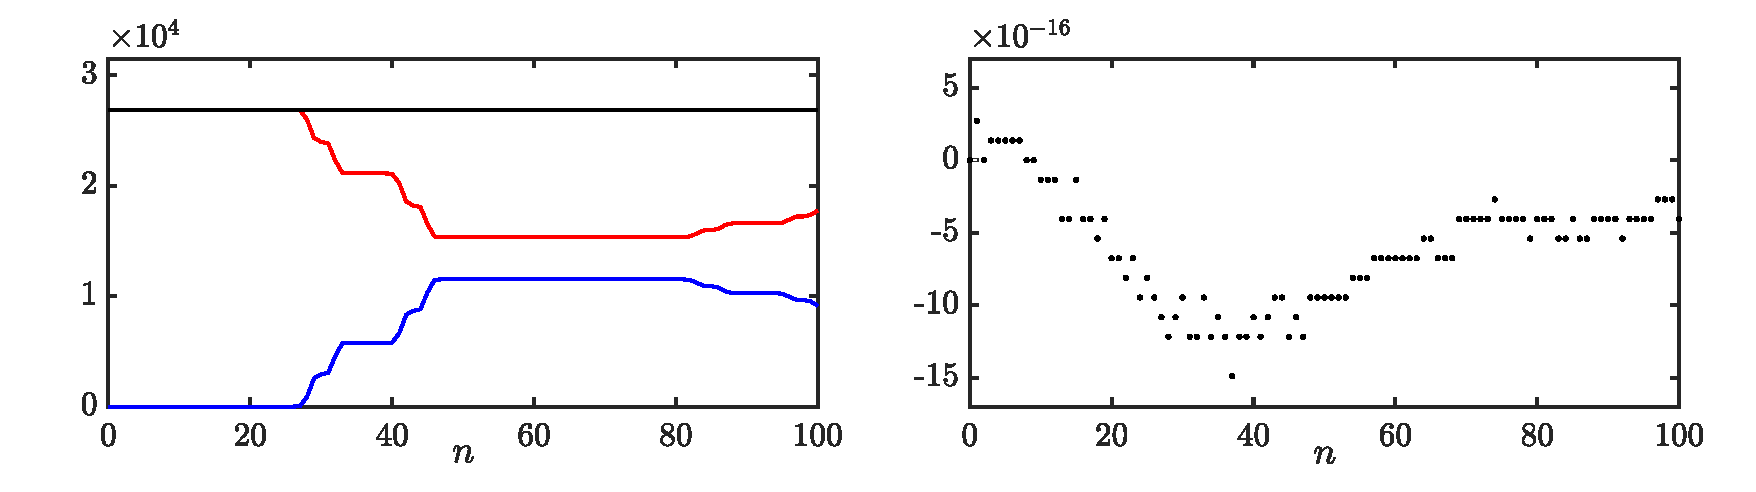
\includegraphics[width=\textwidth]{figures/interactions/connected1DEnergy.eps}
        };
    
        \node[] (he) at (0.2,0.5) {\small $\mathfrak{h}_\text{e}$};

        \node[] (h) at (-5.9, 1) {\small $\mathfrak{h}$};
        \node[] (v) at (-5.9, 0.5) {\small $\color{red}\mathfrak{h}_u$};
        \node[] (t) at (-5.9, 0) {\small $\color{blue}\mathfrak{h}_w$};
      \end{tikzpicture}
      \caption{The energy of $u$ (red), the energy of $w$ (blue), and the total (black) energy of the system of connected 1D wave equations in \eqref{eq:conn1DwaveFDS}. The energy corresponds to Figure \ref{fig:connectedWaveEqs}. The right panel shows the normalised energy (according to Eq. \eqref{eq:normalisedEnergy}) and shows that the deviation of the energy is within machine precision. \label{fig:energyConn1DWave}}
\end{figure}

\subsection{Matrix form}\label{sec:matrixFormRigid}
% In order to perform a modal analysis on the system, one must use the matrix form of the system in Eq. \eqref{eq:conn1DwaveMatrix}. 

One can write the system in Eq. \eqref{eq:conn1DwaveFDS} with a rigid connection in matrix form, albeit slightly more involved due to the interconnection of the schemes.

To start, the definition of the force in Eq. \eqref{eq:rigidForce} must be substituted into the system, which, after expansion of the left hand side of the system, becomes
\begin{subequations}\label{eq:forceExpanded1Dwaves}
    \begin{align}
        &\begin{aligned}
            u_l^{n+1} &= 2\uln - u_l^{n-1} + c^2k^2\dxx \uln \\
            &- \Ju\frac{k^2}{\rho_u A_u} \left(\frac{c_u^2 \Iu\dxx \uln - c_w^2 \Iw\delta_{\chi\chi} \wmn}{\frac{\lVert \Ju\rVert_{d_u}^2}{\rho_u A_u} + \frac{\lVert \Jw\rVert_{d_w}^2}{\rho_w A_w}}\right), 
        \end{aligned}\\
        &\begin{aligned}
            w_m^{n+1} &= 2\wmn - w_m^{n-1} + c^2k^2\dxx \wmn \\
            &+ \Jw\frac{k^2}{\rho_w A_w} \left(\frac{c_u^2 \Iu\dxx \uln - c_w^2 \Iw\delta_{\chi\chi} \wmn}{\frac{\lVert \Ju\rVert_{d_u}^2}{\rho_u A_u} + \frac{\lVert \Jw\rVert_{d_w}^2}{\rho_w A_w}}\right).
        \end{aligned}
    \end{align}
\end{subequations}
Using Dirichlet boundary conditions for both ideal strings, their values can be stored in the following vectors:
\begin{equation*}
    \u^n =[u_1^n, \hdots, u_{N_u-1}^n]^T, \qaq \w^n =[w_1^n, \hdots, w_{N_u-1}^n]^T.
\end{equation*}
These vectors can then be concatenated to one larger state vector, and after the terms in Eqs. \eqref{eq:forceExpanded1Dwaves} are grouped by the grid functions at various time indices, one obtains the following compact matrix form of system \eqref{eq:conn1DwaveFDS}:
\begin{equation}\label{eq:conn1DwaveMatrix} 
    \begin{bmatrix}
        \u^{n+1}\\
        \w^{n+1}
    \end{bmatrix} = \B \begin{bmatrix}
        \u^n\\
        \w^n
    \end{bmatrix} - \begin{bmatrix}
        \u^{n-1}\\
        \w^{n-1}
    \end{bmatrix},
\end{equation}
% \begin{equation}
%     \mathbf{v}^{n+1} = \B \mathbf{v}^n - \mathbf{v}^{n-1}
% \end{equation}
where 
\begin{equation*}
    \B = \begin{bmatrix}
        \B_u & \mathbf{0}\\
        \mathbf{0} & \B_w 
    \end{bmatrix} + \begin{bmatrix}
        -\j_u\\
        \j_w
    \end{bmatrix}
    \begin{bmatrix}
        \mathbf{f}_u& -\mathbf{f}_w
    \end{bmatrix}.
\end{equation*}
The matrix in the definition of $\B$ contains the operations of the 1D wave equation (also see Eq. \eqref{eq:1DwaveMatrix}),
\begin{equation}    
    \B_u = 2\I_{N_u-1} +c_u^2k^2 (\Dxx)_u, \qaq \B_w = 2\I_{N_w-1} +c_w^2k^2 (\Dxx)_w,
\end{equation}
where matrices $(\Dxx)_u$ and $(\Dxx)_w$ are as defined in Eq. \eqref{eq:DxxDef} and are of the appropriate sizes. The vector multiplication in the definition of $\B$ results in a matrix, and adds the effect of the connection force to the system. Here, $\j_u$ and $\j_w$ are column vectors of size $(N_u-1)\times 1$ and $(N_w-1)\times 1$ containing the values of the spreading operators $\Ju$ and $\Jw$ respectively. Finally,
\begin{equation*}
    \mathbf{f}_u = \frac{k^2}{\rho_uA_u} \left(\frac{c_u^2\i_u(\Dxx)_u}{\frac{\i_u \j_u}{ \rho_u A_u} + \frac{\i_w \j_w}{\rho_w A_w}}\right), \qaq \mathbf{f}_w =  \frac{k^2}{\rho_wA_w}\left(\frac{c_w^2 \i_w(\Dxx)_w}{\frac{\i_u \j_u}{ \rho_u A_u} + \frac{\i_w \j_w}{\rho_w A_w}}\right),
\end{equation*}
%are row vectors of size $1\times (N_u-1)$ and $1\times (N_w-1)$, 
where $\i_u$ and $\i_w$ are row vectors of size $1\times (N_u-1)$ and $1\times (N_w-1)$ containing the values of the interpolation operators $\Iu$ and $\Iw$ respectively. Here, $\i_u\j_u$ and $\i_w\j_w$ are matrix-vector forms of $\lVert \Ju\rVert_d^2$ and $\lVert \Jw\rVert_d^2$ respectively (see Eq. \eqref{eq:JnormIJ}) and reduce to a scalar. \todo{check with stefan if this is a correct notation for this}

Equation \eqref{eq:conn1DwaveMatrix} can then easily be rewritten in one-step form as described in Section \ref{sec:oneStepForm} and used for modal analysis.\footnote{As the system does not exhibit damping, it could be analysed directly, not using a one-step form.}
% Following Section \ref{sec:oneStepForm}, one can rewrite Eq. \eqref{eq:conn1DwaveMatrix} to

% \begin{equation}
%     \underbrace{\begin{bmatrix}
%         \u^{n+1}\\
%         \w^{n+1}\\
%         \u^{n}\\
%         \w^{n}
%     \end{bmatrix}}_{\mathbf{v}^{n+1}} = \underbrace{\begin{bmatrix}
%         \B & -\I\\
%         \I,& \mathbf{0}
%     \end{bmatrix}}_{\Q}\underbrace{\begin{bmatrix}
%         \u^{n}\\
%         \w^{n}\\
%         \u^{n-1}\\
%         \w^{n-1}
%     \end{bmatrix}}_{\mathbf{v}^n},
% \end{equation}
% one can insert a test solution $\mathbf{v}^n=z^n\boldPhi$ to get
% \begin{equation*}
%     z\boldPhi = \Q\boldPhi,
% \end{equation*}
% and solved for the $p$\th eigenvalue by following the process in Section \ref{sec:oneStepForm}.

% \todo{figure?}

\section{Spring connection}\label{sec:springConnection}
An alternative connection type is the \textit{spring connection}. As in the rigid case, forces are still equal and opposite, but spring connections allow the relative displacement between the two connected elements to be non-zero. This relative displacement is used to determine the connection force. Interestingly, a nonlinear component can be added to this connection without making the system implicit. The most complex springs used in this project have a linear and a nonlinear (cubic) component, as well as a damping term. For ease of explanation, this section will only use a linear spring. A damped nonlinear spring will appear in Section \ref{sec:stringPlateConnection}. 

The force between two components connected by a linear spring can be defined as
\begin{equation}\label{eq:linearSpringForceCont}
    f = f(t) = K\eta,
\end{equation}
where $K\geq 0$ is the spring constant (in N/m) and
\begin{equation}\label{eq:etaLinSpringCont}
    \eta = \eta(t) = u(x_\ctxt, t) - w(\chi_\ctxt, t)
\end{equation}
is the relative displacement between the two systems at their respective connection locations (in m).\footnote{Note that if $u$ was placed 'below' $w$ (see Section \ref{sec:connIdealStrings}), the signs of the force terms in system \eqref{eq:conn1DwaveFDS} would have been flipped and $u(x_\ctxt, t)$ would have been subtracted from $w(\chi_\ctxt, t)$ in Eq. \eqref{eq:etaLinSpringCont} instead.} 

% This is important for the signs when adding the force terms to the schemes.
%$\eta$ is thus also, effectively, the length of the spring.

In discrete time, Eq. \eqref{eq:linearSpringForceCont} becomes
\begin{equation}\label{eq:linearSpringForceDisc}
    f^n = K\mtd\eta^n,
\end{equation}
where
\begin{equation}\label{eq:discEtaConn1Dwave}
    \eta^n = \Iu\uln - \Iw\wmn.
\end{equation}
Here, the centred averaging operator is used for stability (see Section \ref{sec:conn1DwaveEnergySpring}), but when substituted into system \eqref{eq:conn1DwaveFDSXc} seems to make the system implicit. However, one can find an explicit solution, even for an arbitrary amount of connections \cite{Bilbao2009Modular}. These systems are therefore referred to as being \textit{semi-implicit}, and the process of how to solve the system explicitly will be shown below.

\subsection{Explicit solution}\label{sec:explicitSolutionSpringConn}
Compared to the rigid connection in Section \ref{sec:rigidConn}, solving for $f^n$ requires an extra step. After isolating the schemes at their respective connection locations -- resulting in Eqs. \eqref{eq:conn1DwaveFDSXc} -- one needs to expand the scheme and solve for the states at $n+1$:
\begin{subequations}\label{eq:intermediateConn1Dwave}
    \begin{align}
        \Iu u_l^{n+1} &= u^\star - \lVert\Ju\rVert_{d_u}^2 \frac{k^2f^n}{\rho_u A_u},\\
        \Iw w_m^{n+1} &= w^\star + \lVert\Jw\rVert_{d_w}^2 \frac{k^2f^n}{\rho_w A_w},
    \end{align}
\end{subequations}
where
\begin{equation*}
    u^\star = \Iu(2\uln - u_l^{n-1}) + c_u^2k^2\Iu\dxx\uln,
\end{equation*}
and
\begin{equation*}
    w^\star = \Iw(2\wmn - w_m^{n-1}) + c_w^2k^2\Iw\dxx\wmn,
\end{equation*}
are the update equations of the system at their respective connection locations, without the term containing the connection force (as done in Chapter \ref{ch:collisions}). Evaluating Eq. \eqref{eq:discEtaConn1Dwave} at $n+1$ yields
\begin{equation*}
    \eta^{n+1} = \Iu u_l^{n+1} - \Iw w_m^{n+1},
\end{equation*}
into which Eqs. \eqref{eq:intermediateConn1Dwave} can be substituted, as
\begin{equation}\label{eq:etaNp1Schemes}
    \eta^{n+1} = u^\star - \lVert\Ju\rVert_{d_u}^2 \frac{k^2f^n}{\rho_u A_u} - \left(w^\star + \lVert\Jw\rVert_{d_w}^2 \frac{k^2f^n}{\rho_w A_w}\right).
\end{equation}
A second definition for $\eta^{n+1}$ can be obtained after expanding Eq. \eqref{eq:linearSpringForceDisc}:
\begin{equation}\label{eq:etaExpanded}
    \eta^{n+1} = \frac{2 f^n}{K} - \eta^{n-1}
\end{equation}
and can be substituted into Eq. \eqref{eq:etaNp1Schemes} to get
\begin{equation}
    \frac{2 f^n}{K} - \eta^{n-1} = u^\star - \lVert\Ju\rVert_{d_u}^2 \frac{k^2f^n}{\rho_u A_u} - \left(w^\star + \lVert\Jw\rVert_{d_w}^2 \frac{k^2f^n}{\rho_w A_w}\right).
\end{equation}
Finally, one can group the terms for $f^n$ 
\begin{equation*}
    \left(\frac{2}{K} + \frac{\lVert\Ju\rVert_{d_u}^2k^2}{\rho_u A_u} +  \frac{\lVert\Jw\rVert_{d_w}^2k^2}{\rho_w A_w}\right)f^n = u^\star - w^\star + \eta^{n-1}
\end{equation*}
and solve for the force, solely based on known values of the system
\begin{equation}
    f^n = \frac{u^\star - w^\star + \eta^{n-1}}{\frac{2}{K} + \frac{\lVert\Ju\rVert_{d_u}^2k^2}{\rho_u A_u} +  \frac{\lVert\Jw\rVert_{d_w}^2k^2}{\rho_w A_w}}\ .
\end{equation}

Figure \ref{fig:connectedWaveEqsSpring} shows the behaviour of system Eq. \eqref{eq:conn1DwaveFDS}, connected with a spring with spring constant $K = 5\cdot 10^4$ N/m. The same parameters, excitation and connection locations are used as for the rigid connection in Section \ref{sec:rigidConn}. Compared to the behaviour of the system with a rigid connection in Figure \ref{fig:connectedWaveEqs}, one can observe that the distance between the two connected points gets larger as the wave passes the connection point, which corresponds to the extension of the spring. 
% Furthermore, the transfer of energy from $u$ to $w$ is slower than in the rigid case due to the spring extension (see \ref{sec:energy.

\begin{figure}[h]
    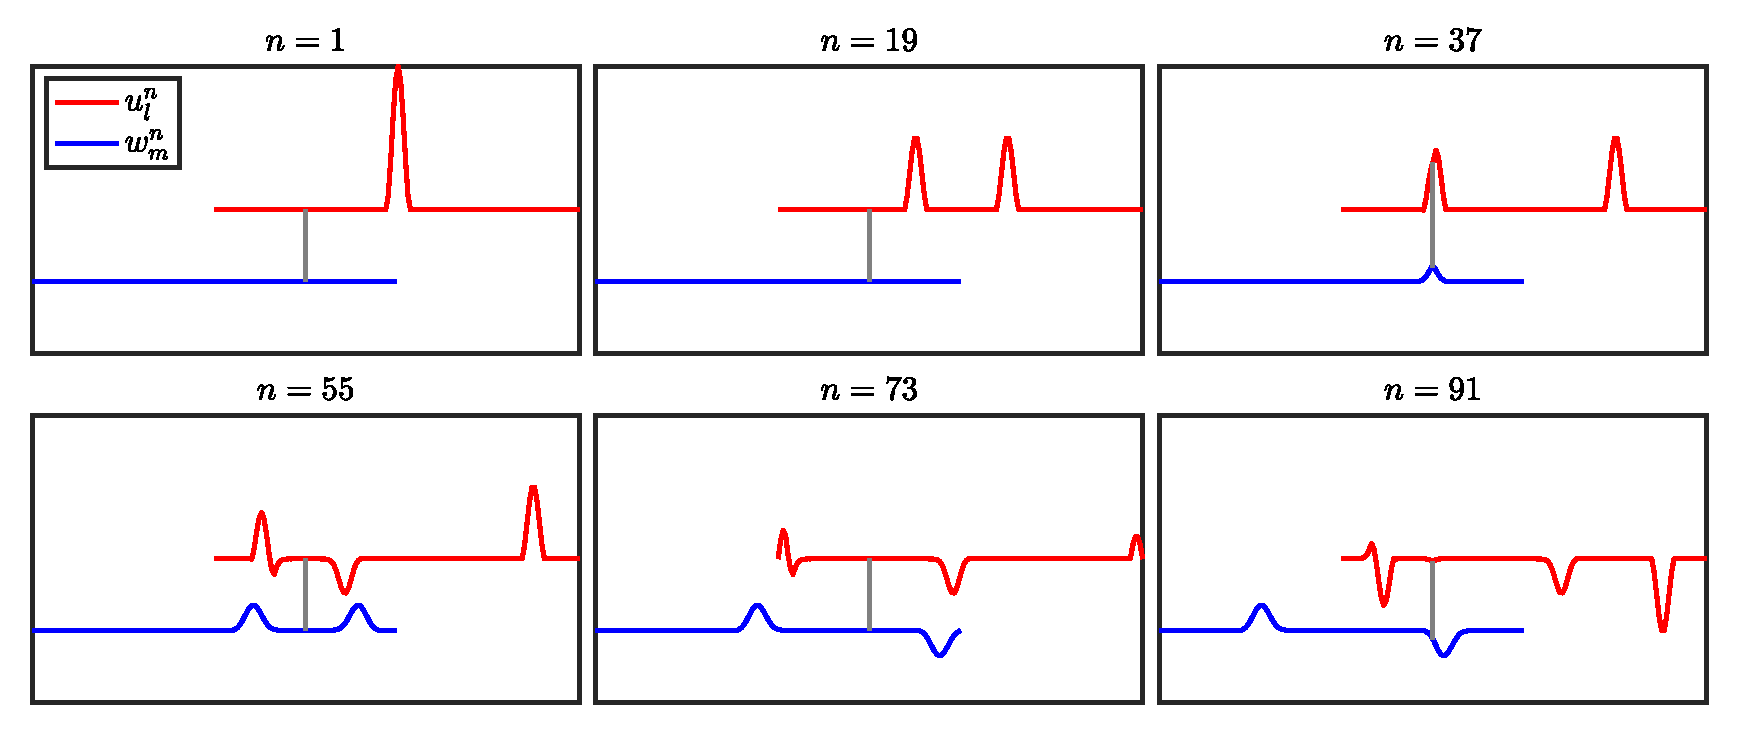
\includegraphics[width=\textwidth]{figures/interactions/connectedWaveEqsSpring.eps}
    \caption{The behaviour of two ideal strings connected using a spring. The systems are offset for clarity, but the relative displacement at the connection location at the start of the simulation is 0. \label{fig:connectedWaveEqsSpring}}
\end{figure}

\subsection{Energy analysis}\label{sec:conn1DwaveEnergySpring}
% As springs store energy themselves, it needs to be shown that stability is maintained.\todo{wording} 
This section follows the energy analysis techniques presented in Section \ref{sec:energyAnalysis} (without explicitly following the steps for brevity) and shows that the discretisation of the spring force chosen in Eq. \eqref{eq:linearSpringForceDisc} is inherently stable. 

Following the same process as in Section \ref{sec:energyAnalysis1DwaveConnRigid}, one can analyse system \eqref{eq:conn1DwaveFDS}, and arrive at Eq. \eqref{eq:rOCconnSystem}:
\begin{equation*}
    \dtp (\h_u + \h_w) = -\Iu \dtd \uln f^n + \Iw \dtd \wmn f^n,
\end{equation*}
which can be rewritten to
\begin{equation*}
    \dtp (\h_u + \h_w) = -\dtd\left(\Iu \uln - \Iw \wmn\right)f^n.
\end{equation*}
One can then substitute the definitions for $f^n$ and $\eta^n$ from Eqs. \eqref{eq:linearSpringForceDisc} and \eqref{eq:discEtaConn1Dwave} to get
\begin{equation}\label{eq:energyAfterForceSubstitution}
    \dtp (\h_u + \h_w) = -K(\dtd \eta^n) (\mtd \eta^n),
\end{equation}
which, using identity \eqref{eq:prodIdentity4}, can be rewritten to
\begin{equation}
    \dtp (\h_u + \h_w + \h_\ctxt) = 0,
\end{equation}
where
\begin{equation}
    \h_\ctxt = \frac{K}{2}\left(\mtm(\eta^n)^2\right)
\end{equation}
is the energy stored by the connection. As this definition is non-negative it does not affect the stability of the system. The spring constant $K$ could potentially be infinitely large, which would effectively reduce the spring connection to a rigid connection presented in Section \ref{sec:rigidConn}.

Figure \ref{fig:energyConn1DWaveSpring} shows the energy of an implementation of system \eqref{eq:conn1DwaveFDS} connected with a spring with spring constant $K=5\cdot 10^4$. other parameters are the same as for the rigid connection in Section \ref{sec:rigidConn}. One can observe that when compared to Figure \ref{fig:energyConn1DWave}, less energy is transferred from $u$ to $w$, and some energy is stored in the spring shown in green. 


\begin{figure}[h]
    \centering
    \begin{tikzpicture}[->,node distance=3cm,
        thick,main node/.style={circle,draw}]
    
        \node[] (image) at (0,0) {
        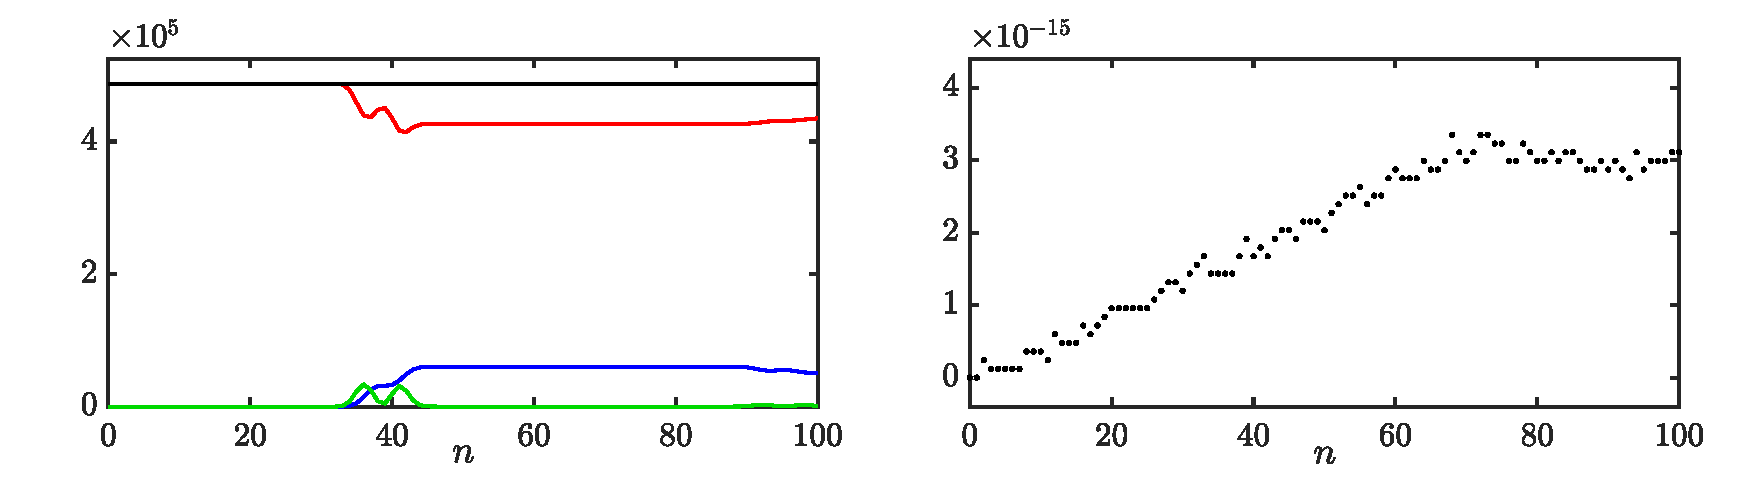
\includegraphics[width=\textwidth]{figures/interactions/connected1DEnergySpring.eps}
        };
    
        \node[] (he) at (0.2,0.5) {\small $\mathfrak{h}_\text{e}$};

        \node[] (h) at (-5.8, 1) {\small $\mathfrak{h}$};
        \node[] (v) at (-5.8, 0.5) {\small $\color{red}\mathfrak{h}_u$};
        \node[] (t) at (-5.8, 0) {\small $\color{blue}\mathfrak{h}_w$};
        \node[] (c) at (-5.8, -0.5) {\small $\color[HTML]{00DB00}\mathfrak{h}_\ctxt$};

      \end{tikzpicture}
      \caption{The energy of $u$ (red), the energy of $w$ (blue), the energy of the spring connection (green) and the total energy (black) of the system of connected 1D wave equations in \eqref{eq:conn1DwaveFDS}. The energy corresponds to the system in Figure \ref{fig:connectedWaveEqsSpring}. The right panel shows the normalised energy (according to Eq. \eqref{eq:normalisedEnergy}) and shows that the deviation of the energy is within machine precision. \label{fig:energyConn1DWaveSpring}}
\end{figure}

\subsubsection{Unstable discretisation}
To show why an averaging operator is used in Eq. \eqref{eq:linearSpringForceDisc}, consider a more straightforward discretisation of Eq. \eqref{eq:linearSpringForceCont} without the averaging operator, such that
\begin{equation*}
    f^n = K\eta^n.
\end{equation*}
Performing an energy analysis of the system would yield 
\begin{equation*}
    \dtp (\h_u + \h_w) = -K(\dtd \eta^n) (\eta^n),
\end{equation*}
(instead of Eq. \eqref{eq:energyAfterForceSubstitution}) and using identity \eqref{eq:prodIdentity2}, this can be rewritten to
\begin{equation*}
    \dtp (\h_u + \h_w + \h_\ctxt) = 0,
\end{equation*}
where
\begin{equation*}
    \h_\ctxt = \frac{K}{2}\left(\eta^ne_{t-}\eta^n\right).
\end{equation*}
As this is not necessarily non-negative, the connection places a larger restriction on the stability of the system at the connection location. In other words, $\lambda \leq 1$ for the ideal strings does not ensure stability at the connection location. Also see \cite[pp. 190--192]{theBible}.

% \section{Spring-like connections}

% Forces are still equal and opposite as the springs are not distributed...

% \subsection{Connection with rigid barrier (scaled)}
% Consider the (scaled) 1D wave equation with an additional force term $F^n$
% \begin{equation}\label{eq:1DwaveConnRigid}
%     \dtt \uln = \gamma^2\dxx \uln + J_l(x_\ctxt)F^n
% \end{equation}
% where
% \begin{equation}\label{eq:1DwaveConnRigidForce}
%     F^n = -\omega_0^2\mtd\eta^n - \omega_1^4(\eta^n)^2\mtd\eta^n - 2\sigma_\times \dtd \eta^n
% \end{equation}
% and
% \begin{equation}\label{eq:etaRigid}
%     \eta^n = I_l(x_\ctxt)\uln.
% \end{equation}

% To obtain $F^n$, an inner product of scheme \eqref{eq:1DwaveConnRigid} needs to be taken with $J_l(x_\ctxt)$ over domain $\D$ which, using identity \eqref{eq:identityIJ} yields 
% \begin{equation}\label{eq:1DwaveConnRigidInnerProd}
%     \dtt I_l(x_\ctxt)\uln = \gamma^2 I_l(x_\ctxt)\dxx \uln + \underbrace{I_l(x_\ctxt)J_l(x_\ctxt)}_{\lVert J_l(x_\ctxt) \rVert^2_\D}F^n.
% \end{equation}
% As $u$ is connected to a rigid barrier according to \eqref{eq:etaRigid}, a shortcut can be taken and Eqs. \eqref{eq:1DwaveConnRigidForce} and \eqref{eq:etaRigid} can be directly substituted into Eq. \eqref{eq:1DwaveConnRigidInnerProd} to get
% \begin{equation}
%     \dtt \eta^n = \gamma^2 I_l(x_\ctxt)\dxx \uln + \lVert J_l(x_\ctxt)\rVert^2_\D\left( -\omega_0^2\mtd\eta^n - \omega_1^4(\eta^n)^2\mtd\eta^n - 2\sigma_\times \dtd \eta^n\right).
% \end{equation}
% and solved for $\eta^{n+1}$:
% \begin{equation}
%     \begin{aligned}
%     &\!\!\!\!\!\!\!\!\!\!\!\!\!\!\Big(1 + \lVert J_l(x_\ctxt)\rVert^2_\D k^2[\omega_0^2/2 + \omega_1^4(\eta^n)^2/2 + \sigma_\times/k] \Big)\eta^{n+1} \\
%    = &\ 2 \eta^n - \Big(1 + \lVert J_l(x_\ctxt)\rVert^2_\D k^2[\omega_0^2/2 + \omega_1^4(\eta^n)^2/2 - \sigma_\times/k]\Big)
%     \eta^{n-1}\\
%     &+ \gamma^2k^2 I_l(x_\ctxt)\dxx\uln
%     \end{aligned}
% \end{equation}
% This can then be used to calculate $F^n$ in \eqref{eq:1DwaveConnRigidForce} and can in turn be used to calculate $u_l^{n+1}$ in \eqref{eq:1DwaveConnRigid}.

\section{String-plate connection}\label{sec:stringPlateConnection}
As an example of a more complicated connected system used in papers \citeP[A] and \citeP[B], consider a stiff string connected to a plate using a nonlinear damped spring. This could be interpreted as a simplified form of how the string would be connected to the body in a stringed instrument. In the following, subscripts `s' and `p' are used to denote a string or plate parameter respectively. 

\subsection{Continuous time}
Consider a damped stiff string of length $L$ (in m), its transverse displacement described by $u = u(\chi,t)$ (in m) defined for $t\geq 0$ and $\chi \in \D_\stxt$ where domain $\D_\stxt = [0, L]$. Its PDE is described by
\begin{equation}
    \rho_\stxt A\ptt u = T \partial_{\chi\chi} u - E_\stxt I \partial_{\chi\chi\chi\chi} u - 2\szX[\stxt]\rho_\stxt A\pt u + 2\soX[\stxt]\rho_\stxt A\pt\partial_{\chi\chi} u,
\end{equation}
where parameters are as in Eq. \eqref{eq:stiffStringPDE}.

The transverse displacement of a damped rectangular thin plate of side lengths $L_x$ and $L_y$ (both in m) can be described as $w=w(x,y,t)$ (in m), which is defined for $t\geq 0$ and $(x,y)\in \D_p$ where domain $\D_p = [0, L_x] \times [0, L_y]$. Its PDE is defined as
\begin{equation}
    \rho_\ptxt H\ptt w = -D\Delta\Delta w - 2\szX[\ptxt]\rho_\ptxt H\pt w + 2\soX[\ptxt] \rho_\ptxt H\pt\pxx w,
\end{equation}
where parameters are as in Eq. \eqref{eq:platePDE}.

One can connect the above PDEs, by adding a localised connection force. After a division by $\rho_\stxt A$ and $\rho_\ptxt H$ respectively the connected string-plate system becomes
\begin{subequations}\label{eq:connStringPlatePDEs}
    \begin{align}
        \!\!\ptt u &= c^2 \partial_{\chi\chi} u - \kappa_\stxt^2 \partial_{\chi\chi\chi\chi} u - 2\szX[\stxt]\pt u + 2\soX[\stxt] \pt\partial_{\chi\chi} u - \delta(\chi-\chi_\ctxt)\frac{f}{\rho_\stxt A},\\
    \!\!\ptt w &= -\kappa_\ptxt^2\Delta\Delta w - 2\szX[\ptxt]\pt w + 2\soX[\ptxt] \pt\pxx w + \delta(x-x_\ctxt, y-y_\ctxt)\frac{f}{ \rho_\ptxt H},
    \end{align}
\end{subequations}
where $\delta(\chi-\chi_\ctxt)$ (in m$^{-1}$) and $\delta(x-x_\ctxt, y-y_\ctxt)$ (in m$^{-2}$) are the 1D and 2D spatial Dirac delta functions defined in Eqs. \eqref{eq:spatialDirac} and \eqref{eq:spatialDirac2D} respectively and locate the connection force at $\chi_\ctxt \in \D_s$ (in m) along the string and $(x_\ctxt,y_\ctxt)\in \D_p$ (in $(\text{m}, \text{m})$) on the plate.

The force between the two components (in N) is set to be a nonlinear (cubic) damped spring defined as (used in e.g. \cite{Webb2015} and in scaled form in \cite{Bilbao2009Modular})
\begin{equation}\label{eq:nonlinearForce}
    f = f(t) = K_1\eta+K_3\eta^3+R \dot\eta,
\end{equation}
with linear and nonlinear spring coefficients $K_1$ (in N/m) and $K_3$ (in N/m$^3$) and damping coefficient $R$ (in kg/s). Furthermore, the distance (in m) between the string and the plate at their respective connection locations is defined as
\begin{equation}
    \eta = \eta(t) = u(\chi_\ctxt, t) - w(x_\ctxt, y_\ctxt, t).
\end{equation}


\subsection{Discrete time}
To discretise $u(\chi, t)$, one can use grid function $\uqn$ where $n\in\mathbb{N}^0$ and $q\in\{0, \hdots, N\}$ with number of grid points $N+1$ (see Section \ref{sec:gridFunctions}). Next, $w(x, y, t)$ can be discretised using grid function $\wlmn$ with $l \in \{0, \hdots, N_x\}$ and $m \in \{0, \hdots, N_y\}$ where $N_x+1$ and $N_y+1$ are the number of grid points in the $x$ and $y$ direction respectively (see Section \ref{sec:2Dintro}). 

Using these grid functions, system \eqref{eq:connStringPlatePDEs} can then be discretised as
\begin{align}\label{eq:connStringPlateFDSs}
    &\begin{aligned}
        \dtt \uqn &= c^2 \dcc \uqn - \kappa_\stxt^2 \dcccc \uqn - 2\szX[\stxt]\dtd \uqn + 2\soX[\stxt] \dtm\dcc \uqn \\
        &\qquad - J_q(\chi_\ctxt)\frac{f^n}{\rho_\stxt A}\ ,
    \end{aligned}\\
    &\begin{aligned}
        \dtt \wlmn &= -\kappa_\ptxt^2\dDelta\dDelta \wlmn - 2\szX[\ptxt]\dtd \wlmn + 2\soX[\ptxt] \dtm\dxx \wlmn \\
        &\qquad + J_{l, m}(x_\ctxt, y_\ctxt)\frac{f^n}{\rho_\ptxt H}\ ,
    \end{aligned}
\end{align}
where $J_q(\chi_\ctxt) = J_{q, o_\stxt} (\chi_\ctxt)$ is a 1D spreading operator of order $o_\stxt$ as defined in Section \ref{sec:interpolationSpreading} and $J_{l, m}(x_\ctxt, y_\ctxt) = J_{(l, m), o_\ptxt}(x_\ctxt, y_\ctxt)$ is a 2D spreading operator of order $o_\ptxt$ as defined in Section \ref{sec:interpolationSpreading2D}. 

The definition of the force in Eq. \eqref{eq:nonlinearForce} can be discretised as\footnote{The second-order averaging operator has been chosen here to show an alternative discretisation of the linear term, but it could be replaced by a centred first-order averaging operator as used in Eq. \eqref{eq:linearSpringForceDisc}.}
\begin{equation}\label{eq:discForceStringPlate}
    f^n = K_1\mtt\eta^n+K_3(\eta^n)^2\mtd\eta^n+R\dtd\eta^n,
\end{equation}
where
\begin{equation}\label{eq:discEtaStringPlate}
    \eta^n = I_q(x_\ctxt)\uqn - I_{l, m}(x_\ctxt, y_\ctxt)\wmn.
\end{equation}
Here, $I_q(\chi_\ctxt) = I_{q, o_\stxt} (\chi_\ctxt)$ and $I_{l, m}(x_\ctxt, y_\ctxt) = I_{(l, m), o_\ptxt}(x_\ctxt, y_\ctxt)$ are interpolation operators of the same order as $J_q(\chi_\ctxt)$ and $J_{l,m}(x_\ctxt)$ respectively. 


\subsection{Solving for $f$}
Following the same process as in Section \ref{sec:explicitSolutionSpringConn}, system \eqref{eq:connStringPlateFDSs} needs to be isolated at the connection locations. This is done by taking an inner product of the schemes in \eqref{eq:connStringPlateFDSs} with their respective spreading operators over discrete domains $d_u = \{0, \hdots, N\}$ and $d_w = \{0, \hdots, N_x\}\times \{0, \hdots, N_y\}$ respectively. Taking these inner products, expanding the $\dtt$ and $\dtd$ operators (as these contain $u_q^{n+1}$) and solving for the states at $n+1$ yields
\begin{subequations}\label{eq:connStringPlateFDSsAtConn}
    \begin{align}
        \Iq u_q^{n+1} &= u^\star- \lVert J_q(\chi_\ctxt)\rVert_{d_u}^2\frac{k^2f^n}{\rho_\stxt A(1+\szX[\stxt]k)}\ ,\\
        \Ilm w_{l,m}^n &= w^\star+ \lVert J_{l, m}(x_\ctxt, y_\ctxt)\rVert_{d_w}^2\frac{k^2f^n}{\rho_\ptxt H(1+\szX[\ptxt]k)}\ ,
    \end{align}
\end{subequations}
where
\begin{subequations}
\begin{align}
    &\begin{aligned}
        u^{\star} =&\ \Big(\Iq (2\uqn - u_q^{n-1}) + c^2k^2 \Iq\dcc \uqn - \kappa_\stxt^2k^2 \Iq\dcccc \uqn\\
        &\quad+ \szX[\stxt]k\Iq u_q^{n-1} + 2\soX[\stxt]k^2 \Iq\dtm\dcc \uqn\Big) / (1+\szX[\stxt]k),
    \end{aligned}\label{eq:stringPlateUStar}\\
    &\begin{aligned}
        w^\star =&\ \Big(-\kappa_\ptxt^2\Ilm\dDelta\dDelta \wlmn + \szX[\ptxt]k\Ilm w_{l,m}^{n-1} \\
        &\qquad\qquad+ 2\soX[\ptxt] \Ilm\dtm\dxx \wlmn\Big)/(1+\szX[\ptxt]k),
    \end{aligned}\label{eq:stringPlateWStar}
\end{align}
\end{subequations}
are the update equations of the schemes at their respective connection locations without the force term. 

Evaluating Eq. \eqref{eq:discEtaStringPlate} at $n+1$ and substituting Eqs. \eqref{eq:connStringPlateFDSsAtConn} yields
\begin{equation}\label{eq:etaNextStringPlate1}
    \begin{aligned}
    \eta^{n+1} =&\ u^\star- \lVert J_q(\chi_\ctxt)\rVert_{d_u}^2\frac{k^2f^n}{\rho_\stxt A(1+\szX[\stxt]k)} \\
    &- \left(w^\star + \lVert J_{l, m}(x_\ctxt, y_\ctxt)\rVert_{d_w}^2\frac{k^2f^n}{\rho_\ptxt H(1+\szX[\ptxt]k)}\right).
    \end{aligned}
\end{equation}
Then expanding Eq. \eqref{eq:discForceStringPlate} to
\begin{equation*}
     f^n = \underbrace{\left(\frac{K_1}{4}+\frac{K_3(\eta^n)^2}{2} + \frac{R}{2k}\right)}_{r_+^n}\eta^{n+1} + \frac{K_1}{2}\eta^n + \underbrace{\left(\frac{K_1}{4}+\frac{K_3(\eta^n)^2}{2} - \frac{R}{2k}\right)}_{r_-^n}\eta^{n-1},
\end{equation*}
and solving for $\eta^{n+1}$ yields
\begin{equation}
    \eta^{n+1} = \frac{f^n}{r_+^n} - \frac{K_1}{2r_+^n}\eta^n - \frac{r_-^n}{r_+^n}\eta^{n-1}.
\end{equation}
Substituting this into Eq. \eqref{eq:etaNextStringPlate1}, one can find a definition for the connecting force
\begin{equation}\label{eq:stringPlateForce}
    f^n = \frac{u^\star - w^\star + \frac{K_1}{2r_+^n}\eta^n + \frac{r_-^n}{r_+^n}\eta^{n-1}}{\frac{1}{r_+^n} + \frac{\lVert J_q(\chi_\ctxt)\rVert_{d_u}^2k^2}{\rho_\stxt A(1+\szX[\stxt]k)} + \frac{\lVert J_{l, m}(x_\ctxt, y_\ctxt)\rVert_{d_w}^2k^2}{\rho_\ptxt H(1+\szX[\ptxt]k)}}\ .
\end{equation}

\subsection{Implementation}\label{sec:implementationStringPlate}
This section shows an example of an implementation of the string-plate system. The parameters for the stiff string can be found in Table \ref{tab:stiffStringParams} (with $L = 1.5$ m and $T = 555$ N) and for the thin plate in Table \ref{tab:thinPlateParams} (with $H=5\cdot10^{-4}$). Both systems use simply supported boundary conditions. Additional parameters used for the connection are
\begin{equation*}
    K_1 = 10^4\ \,\text{N/m}, \quad K_3 = 10^7\ \,\text{N/m}^3, \qaq R = 10\ \,\text{kg/s}.
\end{equation*}
The \texttt{MATLAB} code of the implementation can be found online \cite{stringPlateGist}.\footnote{Note that in the online code, $L$, $L_x$ and $L_y$ have been halved to reduce computations and avoid crashes on some machines.}  Figure \ref{fig:stringPlate} shows a visualisation of the string plate system excited with a raised cosine. 
\begin{figure}[h]
    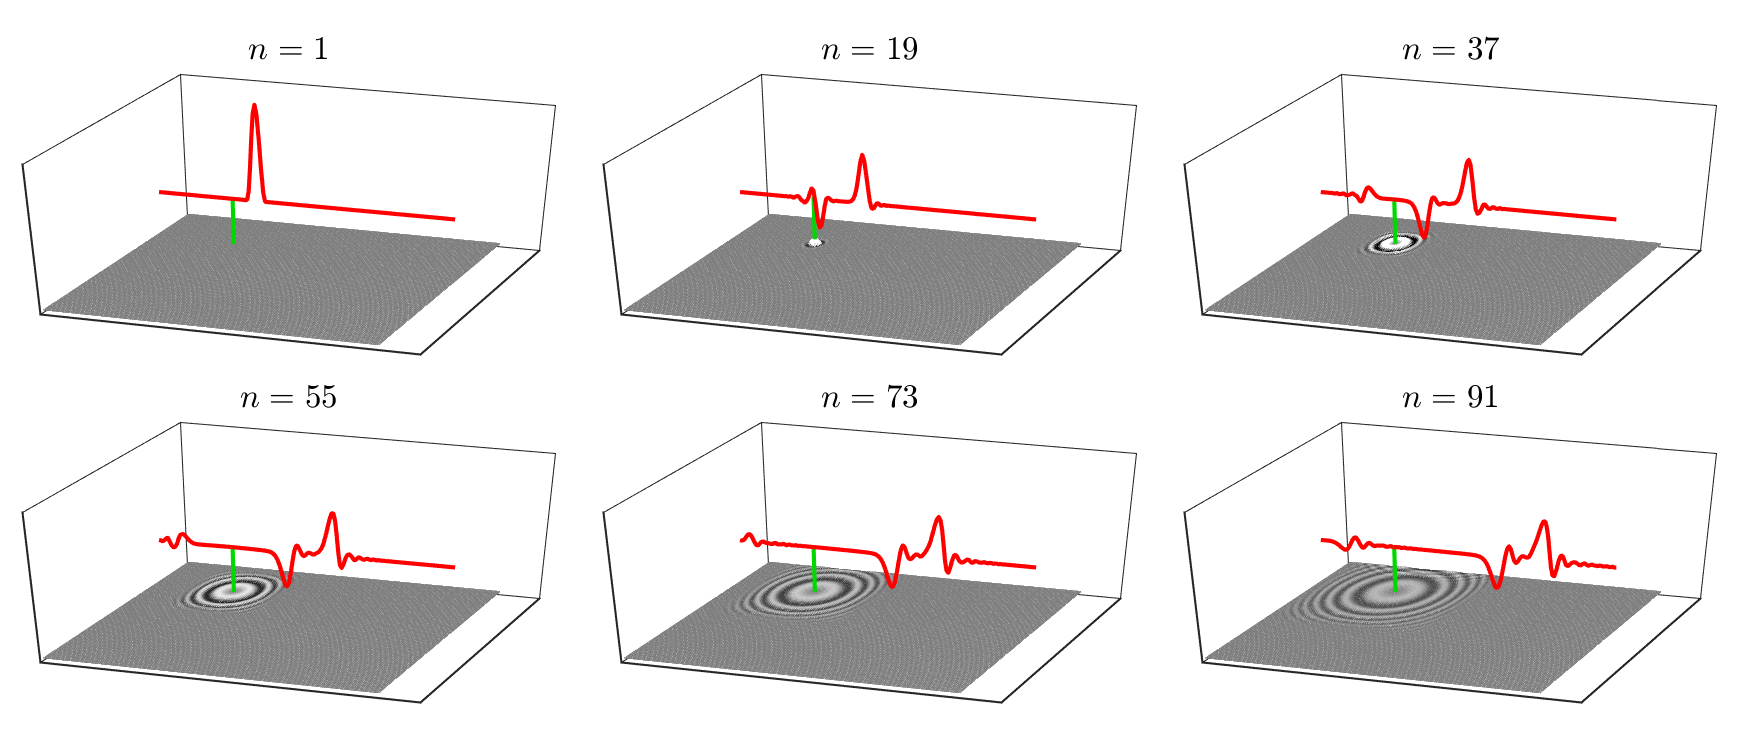
\includegraphics[width=\textwidth]{figures/interactions/stringPlate.eps}
    \caption{The behaviour of the string-plate system connected with a nonlinear damped spring. The string is shown in red, the plate in gray and the connection in green. \label{fig:stringPlate}}
\end{figure}

In the following, the $\i$ and $\j$ vectors are used as in Section \ref{sec:matrixFormRigid} and are of the appropriate sizes. The matrices for the string can be found in Eq. \eqref{eq:matrixFormStiffString} and those for the plate in Eq. \eqref{eq:matrixFormThinPlate}. When implementing connections (or any other interactions for that matter), one mostly performs the following steps in the main loop:
\begin{enumerate}
    \item Calculate the entire scheme without force terms:\\
    \vspace{-0.5em}\begin{equation}\label{eq:stringPlateImp1}
        \u^\star = \frac{\B_\stxt\u^n + \C_\stxt\u^{n-1}}{A_\stxt}, \qaq \w^\star = \frac{\B_\ptxt\w^n + \C_\ptxt\w^{n-1}}{A_\ptxt}\ .
    \end{equation}
    \item Obtain $u^\star$ and $w^\star$:\\
    \vspace{-1em}\begin{equation}\label{eq:stringPlateImp2}
       u^\star = \i_u \u^\star \qaq w^\star = \i_w \w^\star.
    \end{equation}
    \item Calculate the connection force $f^n$ (Eq. \eqref{eq:stringPlateForce}).
    \item Add force terms to the schemes in Eq. \eqref{eq:stringPlateImp1}:\\
    \begin{equation}\label{eq:stringPlateImp4}
        \u^{n+1} = \u^{\star} - \j_u \frac{f^n k^2}{\rho_\stxt A (1+\szX[\stxt])},\qaq \w^{n+1} = \w^{\star} + \j_w \frac{f^n k^2}{\rho_\ptxt H (1+\szX[\ptxt])}.
    \end{equation} 
\end{enumerate}
Calculating $\u^\star$ and $\w^\star$ beforehand reduces computations, and allows $u^\star$ and $w^\star$ to be more easily obtained. 

\subsection{Energy analysis}
Recalling the total energy and damping terms for the string and plate in Sections \ref{sec:energyAnalysisString} and \ref{sec:energyAnalysisThinPlate} respectively, one can --  similar to Eq. \eqref{eq:rOCconnSystem} -- arrive at the following:
\begin{equation}
    \dtp(\h_\stxt + \h_\ptxt) + \q_\stxt + \q_\ptxt = -\Iq (\dtd \uqn)f^n +\Ilm(\dtd \wlmn)f^n,
\end{equation}
which can be rewritten to
\begin{equation*}
    \dtp(\h_\stxt + \h_\ptxt) + \q_\stxt + \q_\ptxt = -\dtd \left(\Iq \uqn - \Ilm\wlmn\right)f^n.
\end{equation*}
Substituting the definitions for $f^n$ and $\eta^n$ from Eqs. \eqref{eq:discForceStringPlate} and \eqref{eq:discEtaStringPlate} respectively, yields
\begin{equation*}
    \dtp(\h_\stxt + \h_\ptxt) + \q_\stxt + \q_\ptxt = -(\dtd\eta^n)(K_1\mtt\eta^n+K_3(\eta^n)^2\mtd\eta^n+R\dtd\eta^n).
\end{equation*}
Due to the nonlinear dependency on $\eta^n$ one must isolate $\dtp$ from the cubic term manually, according to
\begin{align*}
    &\ \ K_3(\eta^n)^2(\dtd \eta^n)(\mtd \eta^n)\\
    = &\ \ \frac{K_3(\eta^2)}{2k}(\eta^{n+1} - \eta^{n-1})\frac{1}{2}(\eta^{n+1} + \eta^{n-1})\\
    = &\ \ \frac{K_3(\eta^n)^2}{4k}\left((\eta^{n+1})^2 - (\eta^{n-1})^2\right)\\
    = &\ \ \frac{K_3}{4k}\left((\eta^{n+1}\eta^n)^2 - (\eta^n\eta^{n-1})^2\right)\\
    = &\ \ \dtp\left(\frac{K_3}{4}(\eta^n\eta^{n-1})^2\right).
\end{align*}
% \begin{equation*}
%     (\dtd \eta^n)K_1\mtt\eta^n \quad \xRightarrow{\text{Eq. \eqref{eq:prodIdentity5}}} \quad \frac{K_1}{8}(\eta^n+\eta^{n-1})^2 
% \end{equation*}
Finally, using identity \eqref{eq:prodIdentity5} for the linear term, the following balance follows
\begin{equation}
    \dtp(\h_\stxt + \h_\ptxt + \h_\ctxt) = - \q_\stxt - \q_\ptxt - \q_\ctxt,
\end{equation}
where the energy stored by the spring connection is
\begin{equation*}
    \h_\ctxt = \frac{K_1}{8}(\eta^n+\eta^{n-1})^2 + \frac{K_3}{4}(\eta^n\eta^{n-1})^2,
\end{equation*}
and the damping term of the connection is
\begin{equation*}
    \q_\ctxt = R(\dtd\eta^n)^2.
\end{equation*}
Figure \ref{fig:energyStringPlate} shows the energetic output of the string-plate system corresponding to the behaviour in Figure \ref{fig:stringPlate}. One can observe that energy is transferred from the string to the plate due to the connection. Furthermore, due to the high value for spring-damping $R$, the total energy decreases substantially as the excitation reaches the connection location along the string. 

\begin{figure}[h]
    \centering
    \begin{tikzpicture}[->,node distance=3cm,
        thick,main node/.style={circle,draw}]
    
        \node[] (image) at (0,0) {
        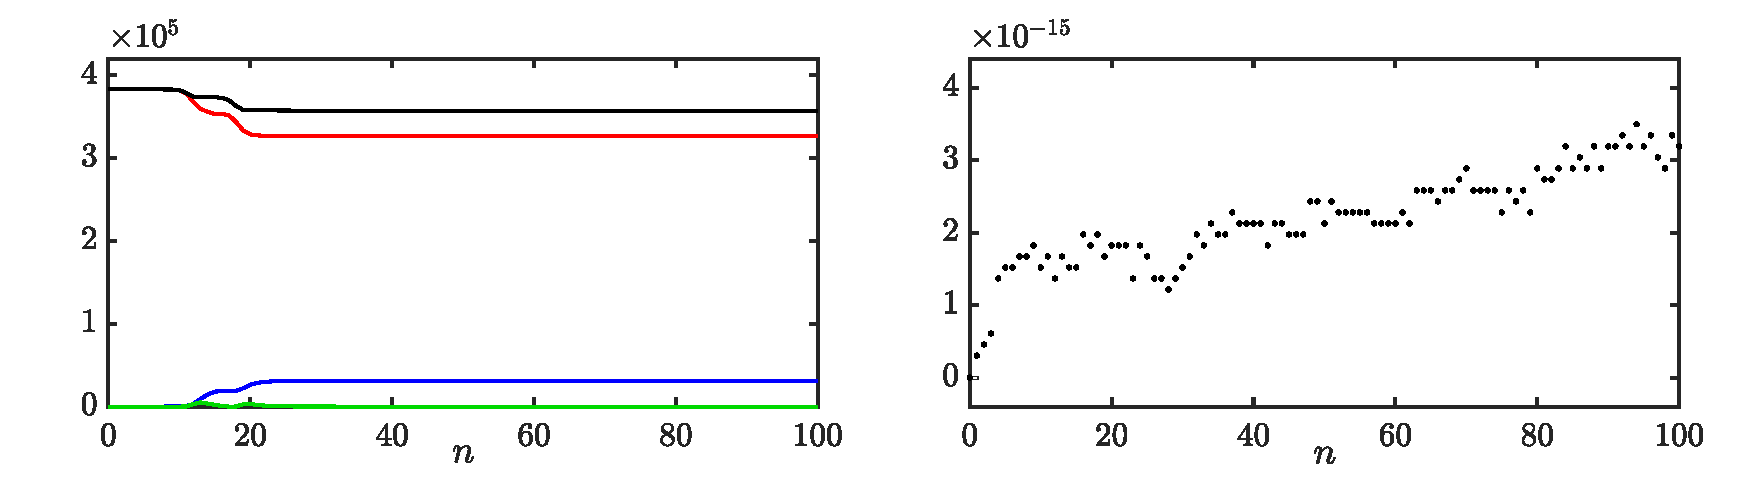
\includegraphics[width=\textwidth]{figures/interactions/stringPlateEnergy.eps}
        };
    
        \node[] (he) at (0.2,0.5) {\small $\mathfrak{h}_\text{e}$};

        \node[] (h) at (-5.8, 1) {\small $\mathfrak{h}$};
        \node[] (v) at (-5.8, 0.5) {\small $\color{red}\mathfrak{h}_\stxt$};
        \node[] (t) at (-5.8, 0) {\small $\color{blue}\mathfrak{h}_\ptxt$};
        \node[] (c) at (-5.8, -0.5) {\small $\color[HTML]{00DB00}\mathfrak{h}_\ctxt$};

      \end{tikzpicture}
      \caption{The energy of the string (red), the plate (blue), the spring connection (green) and the total energy (black) of the connected string-plate system \eqref{eq:connStringPlateFDSs}. The energy corresponds to the system in Figure \ref{fig:stringPlate}. The right panel shows the normalised energy (according to Eq. \eqref{eq:normalisedEnergyDamping}) and shows that the deviation of the energy is within machine precision. \label{fig:energyStringPlate}}
\end{figure}

% \subsection{Non-dimensional}
% The scaled system can be written as:
% \begin{align}
%     \ptt u &= \gamma^2 \pxx u - \kappa_\stxt^2 \pxxxx u - 2\szX[\stxt]\pt u + 2\soX[\stxt] \pt\pxx u - \delta(x-x_\ctxt)F\\
%    \pt w &= -\kappa_\ptxt^2\Delta\Delta w - 2\szX[\ptxt]\pt w + 2\soX[\ptxt] \pt\pxx w + \delta(x-x_\ctxt, y-y_\ctxt)F
% \end{align}
% where
% \begin{equation}
%     F = F(t) = \omega_1^2\eta+\omega_3^4\eta^3+\sigma_\ctxt \dot\eta
% \end{equation}
% and
% \begin{equation}
%     \eta = \eta(t) = u(x_\ctxt, t) - w(x_\ctxt, y_\ctxt, t)
% \end{equation}


% \begin{equation}
%     I(x_\ctxt)\delta_{tt}\uqn = c^2
%     \left(I(x_\ctxt)\dxx\uqn\right) + I(x_\ctxt)J(x_\ctxt)F
% \end{equation}


% \subsubsection{Relative location of objects}\todo{look at this compared to when I talk about it in chapter \ref{ch:collisions}}


% Forces should be equal and opposite. 